\documentclass[conference]{IEEEtran}
\IEEEoverridecommandlockouts

\usepackage{cite}
\usepackage{amsmath,amssymb}
\usepackage{booktabs}
\usepackage{graphicx}
\usepackage{url}

\usepackage{tikz}
\usepackage{graphicx}
\usetikzlibrary{positioning,calc}

\usepackage{hyperref}
\usepackage{xurl}

\usepackage{placeins}


\graphicspath{{../../results/start_2021-01-01_cutoff_2023-01-01_end_2024-12-31/}}

\begin{document}

\title{AI Anxiety Map: Geographic and Emotion Analysis of Global Labor-Market News, 2021–2024}

\author{
\IEEEauthorblockN{Amit Ner Gaon}
\IEEEauthorblockA{
\textit{Department of Software and Information Systems Engineering} \\
\textit{Ben-Gurion University of the Negev} \\
Beer-Sheva, Israel \\
amitner@post.bgu.ac.il}
}

\maketitle

\begin{abstract}
Generative artificial intelligence (AI) has intensified debate about job
displacement and new economic opportunities, but global evidence about how
this debate is framed remains limited. This study analyzes labor-market news
in the GDELT Global Knowledge Graph \cite{leetaru2013gdelt} from 2021 through 2024. It compares two
equal periods before and after AI breakthrough at January 1, 2023 using anxiety and opportunity scores
constructed from global content sentiment analysis, geographic summaries, and
location-emotion similarity networks. Aggregated location-theme article
occurrences increased by 13.9\% after the AI cutoff, while mean anxiety and
opportunity scores each decreased by about 6.9\%. This global reduction was
not geographically uniform: anxiety increased in 122 of 197 countries 
and in 46 of 50 U.S. states. Country changes in anxiety and
opportunity were positively correlated ($r=0.57$), indicating that they often
represent common variation in emotional intensity rather than opposite ends
of one scale. Among 18 high-volume locations shared by both network periods,
mean pairwise emotional similarity decreased by 1.5\%, with 80 pairs
converging and 73 diverging. The findings demonstrate the value of combining
temporal, geographic, and network views, for large scale emotion analysis.

Code is available at:\\ 
\href{https://github.com/AmitNG2000/Data-Mining-Assignments} {\texttt{github.com/AmitNG2000/Data-Mining-Assignments}}.
\end{abstract}

\begin{IEEEkeywords}
generative AI, labor market, GDELT, emotion analysis, geographic analysis,
network analysis, News
\end{IEEEkeywords}

\section{Introduction}

Generative AI can automate parts of knowledge work while also complementing
workers and creating new tasks. Research on the history of automation describes 
the same broader tension: technology replaces some tasks, 
increases the value of complementary skills, 
and distributes adjustment costs unevenly \cite{autor2015jobs, acemoglu2020robots}.
Recent research reports productivity gains from generative AI 
across a wide range of workplace tasks \cite{noy2023experimental,brynjolfsson2025generative}.
These productivity gains often raise concerns about job displacement, 
downward pressure on wages, and the obsolescence of existing skills.


News media provide a large, time-stamped record that can serve as an
proxy for the concerns, priorities, and emotional responses expressed within communities \cite{ploger2025relationships}. 
Although news coverage does not directly measure public opinion or workers’ experiences, 
it enables large-scale and systematic collection of discourse data across countries, 
as well as comparative sentiment and emotion analysis. 
Prior research has shown that news coverage of AI combines persistent optimism 
with growing concern about ethics, control, and employment \cite{fast2017long}. 
This research extends this approach to a multinational news and 
models geographic variation and cross-location similarity.

January 1, 2023 is used as an operational marker for the rapid diffusion of generative AI: 
ChatGPT was released in late 2022, GPT-4 followed in March 2023, 
and generative-AI tools achieved substantial organizational adoption during 2023 
\cite{openai2022chatgpt,openai2023gpt4,mckinsey2023genai}.



This study addresses three research questions:
\begin{enumerate}
\item \textbf{RQ1:} How did anxiety, opportunity, and overall sentiment framing of the
global labor-market differ between the BEFORE AI and AFTER AI periods?

\item \textbf{RQ2:} How did the emotional framing of the labor-market vary
across countries between the BEFORE AI and AFTER AI periods?

\item \textbf{RQ3:} How similar or polarized were locations in their
emotional framing of labor-market, and how did these relationships
change between the BEFORE AI and AFTER AI periods?

\end{enumerate}


This study presents a reproducible framework combining emotion analysis, 
temporal comparisons, geographic summaries, and similarity networks.

\section{Related Work}

Recent studies show that generative AI can increase productivity by 
improving both the speed and quality of work. 
These benefits vary across tasks and workers, with particularly strong gains among 
less-experienced employees \cite{noy2023experimental,brynjolfsson2025generative}.

At the same time, public attitudes toward AI include substantial concern about employment risk. 
Survey evidence from 16 Latin American countries shows that fear of job loss 
due to AI varies over time and across countries \cite{cremaschi2025will}.

Although it does not directly measure public opinion, 
content analysis of digital discourse can reveal how AI is emotionally framed on the public. 
Research on Reddit discussions identifies both optimism and “algorithmic anxiety” 
related to job displacement, professional identity, 
and trust in employers \cite{shekhar2026algorithmic}. 
Similarly, an analysis of \texttt{The New York Times} found that 
AI coverage was generally more optimistic than pessimistic, 
while concerns about employment, ethics, and loss of control increased 
over time \cite{fast2017long}.

\section{Methodology}

\subsection{Collection and Aggregation}

The pipeline processes both the original-language and translated 
streams of the GDELT 2.1 Global Knowledge Graph (GKG).
A record is retained when its structured \texttt{V2Themes} field 
contains at least one predefined labor-market theme, such as employment, 
unemployment, jobs, workers, hiring, layoffs, wages, income, careers, unions, 
gig work, or freelance work. 
For each retained record, the pipeline extracts the publication date, 
matched themes, location, tone, and emotions. 

Because a single GKG record may mention multiple locations and
match multiple labor-market themes, the pipeline creates one observation
for each location--theme combination.
These observations are then aggregated into seven-day intervals by location,
country code, administrative code, and theme.
Accordingly, \texttt{article\_count} represents the number of grouped record
occurrences rather than the number of globally unique articles.

\subsection{Emotional Scores and Period Comparison}

GDELT’s Global Content Analysis Measures (GCAM) apply multiple dictionary-based 
content-analysis systems to news articles, including LIWC and WordNet-Affect, 
to identify emotional and cognitive language. 
LIWC classifies words into psychologically meaningful categories, 
while WordNet-Affect organizes words and concepts associated 
with emotions such as anxiety and fear 
\cite{tausczik2010psychological,strapparava2004wordnet,gdeltgkg2015Codebook}. 

For aggregate row $i$, the anxiety score is calculated as the mean of the available LIWC anxiety, 
WordNet-Affect anxiety, WordNet-Affect fear, and GCAM c6.6 uncertainty dimensions:

\begin{equation}
A_i=\frac{1}{|\mathcal{N}_i|}\sum_{d\in\mathcal{N}_i}x_{i,d}.
\end{equation}
The opportunity score averages the available WordNet hope and optimism
dimensions:
\begin{equation}
O_i=\frac{1}{|\mathcal{Q}_i|}\sum_{d\in\mathcal{Q}_i}x_{i,d}.
\end{equation}
The anxiety-opportunity gap is $F_i=A_i-O_i$.

Rows whose window starts before January 1, 2023 are assigned to the before-AI
period, and all later rows to the after-AI period. Global differences are
assessed with Welch tests, while weekly series are used to inspect whether a
period average conceals trends or peaks. Country and U.S. state summaries are
computed only for units observed with both scores in both periods. Pearson
correlation between country-level changes in $A$ and $O$ are evaluated.

\subsection{Location-Emotion Networks}

For each period, a weighted bipartite graph links up to 20 countries with the
largest interaction volumes to nine GCAM emotion dimensions. An edge weight
is the mean score for that location-emotion combination. The projected
similarity between locations $u$ and $v$ is
\begin{equation}
S(u,v)=\sum_{e\in E(u)\cap E(v)}\min\{w(u,e),w(v,e)\},
\end{equation}
where $w(u,e)$ is the bipartite edge weight. This overlap measure is larger
when two locations share emotions at similar intensities.

\begin{figure}[t]
    \centering
    \resizebox{\columnwidth}{!}{
    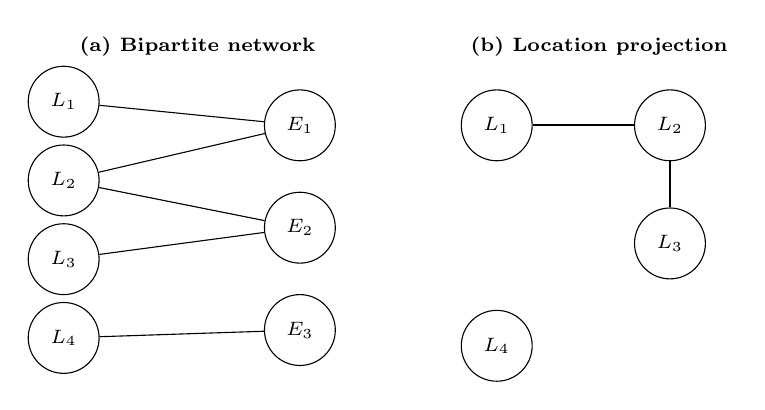
\begin{tikzpicture}[
        font=\scriptsize,
        graphnode/.style={
            circle,
            draw,
            minimum size=9mm,
            inner sep=0pt,
            align=center
        },
        connection/.style={draw, thin},
        projection/.style={draw, thick}
    ]

    % Panel A: Bipartite graph
    \node[font=\scriptsize\bfseries] at (1.7,3.1)
        {(a) Bipartite network};

    % Location nodes
    \node[graphnode] (l1) at (0,2.4) {$L_1$};
    \node[graphnode] (l2) at (0,1.4) {$L_2$};
    \node[graphnode] (l3) at (0,0.4) {$L_3$};
    \node[graphnode] (l4) at (0,-0.6) {$L_4$};

    % Emotion nodes
    \node[graphnode] (e1) at (3,2.1) {$E_1$};
    \node[graphnode] (e2) at (3,0.8) {$E_2$};
    \node[graphnode] (e3) at (3,-0.5) {$E_3$};

    % Bipartite edges
    \draw[connection] (l1) -- (e1);
    \draw[connection] (l2) -- (e1);
    \draw[connection] (l2) -- (e2);
    \draw[connection] (l3) -- (e2);
    \draw[connection] (l4) -- (e3);

    % Panel B: Location projection
    \node[font=\scriptsize\bfseries] at (6.8,3.1)
        {(b) Location projection};

    \node[graphnode] (p1) at (5.5,2.1) {$L_1$};
    \node[graphnode] (p2) at (7.7,2.1) {$L_2$};
    \node[graphnode] (p3) at (7.7,0.6) {$L_3$};
    \node[graphnode] (p4) at (5.5,-0.7) {$L_4$};

    % Projection edges
    % L1 and L2 share E1
    \draw[projection] (p1) -- (p2);

    % L2 and L3 share E2
    \draw[projection] (p2) -- (p3);

    % L4 is isolated because no other location shares E3

    \end{tikzpicture}
    }
    \caption{
        Bipartite location--emotion network and its one-mode location projection.
        Two locations are connected in the projection if they share at least one
        emotion in the bipartite graph.
    }
    \label{fig:bipartite_projection}
\end{figure}

Figure~\ref{fig:bipartite_projection} illustrates the projection of the
location--emotion bipartite network onto a location-only network.
Two locations are connected when both are associated with at least one
common emotion.

\subsection{Temporal Analysis}

Temporal variation is examined at the same seven-day resolution used during
data aggregation. For each location and interval, article occurrences and
interactions are summed across labor-market themes, while anxiety and
opportunity are calculated as the arithmetic means of the available
location--theme scores. The global time series is then constructed by summing
article occurrences and averaging the location-level scores within each
interval.

Weekly anxiety and opportunity series are plotted with January 1, 2023 marked
as the boundary between the two study periods. The series are inspected for
trends, short-lived peaks, and whether any change near the cutoff is sustained.
For geographic comparisons, each country's and U.S. state's mean score is
calculated separately for the before- and after-AI periods, and temporal change
is defined as the after-period mean minus the before-period mean.


\section{Experiments and Results}

\subsection{system Configuration}

The production run covers January 1, 2021 through December 31, 2024, split
into equal two-year periods. 
The analysis is implemented in Python 3.11 with
pandas, SciPy, NetworkX, Matplotlib, Plotly, and PyDeck. 
Large-scale collection and notebook execution were run on the Ben-Gurion
University Slurm cluster using CPUs.

\subsection{Data}

This study uses the GDELT 2.1 Global Knowledge Graph (GKG), 
a continuously updated international news database 
containing structured information on themes, locations, tone, and events 
\cite{leetaru2013gdelt,gdeltgkg2015Codebook}. 
Its multilingual coverage, translated news stream, and GCAM emotion variables 
enable consistent cross-country analysis of labor-market discourse at a 
large scale.
For this research, the data spans January 2021 to December 2024, 
providing two equal periods before and after the January 1, 2023 cutoff.


\subsection{RQ1: Global Emotional Framing}

\begin{table}[t]
\caption{Global before-after summary}
\label{tab:global}
\centering
\small
\begin{tabular}{lrrrr}
\toprule
Period & Occurrences & $A$ & $O$ & $F$ \\
\midrule
Before AI & 718.9M & 6.341 & 2.785 & 4.617 \\
After AI  & 818.8M & 5.902 & 2.592 & 4.225 \\
Change (\%) & +13.9 & -6.9 & -6.9 & -8.5 \\
\bottomrule
\end{tabular}
\end{table}

\begin{figure*}[!t]
\centering
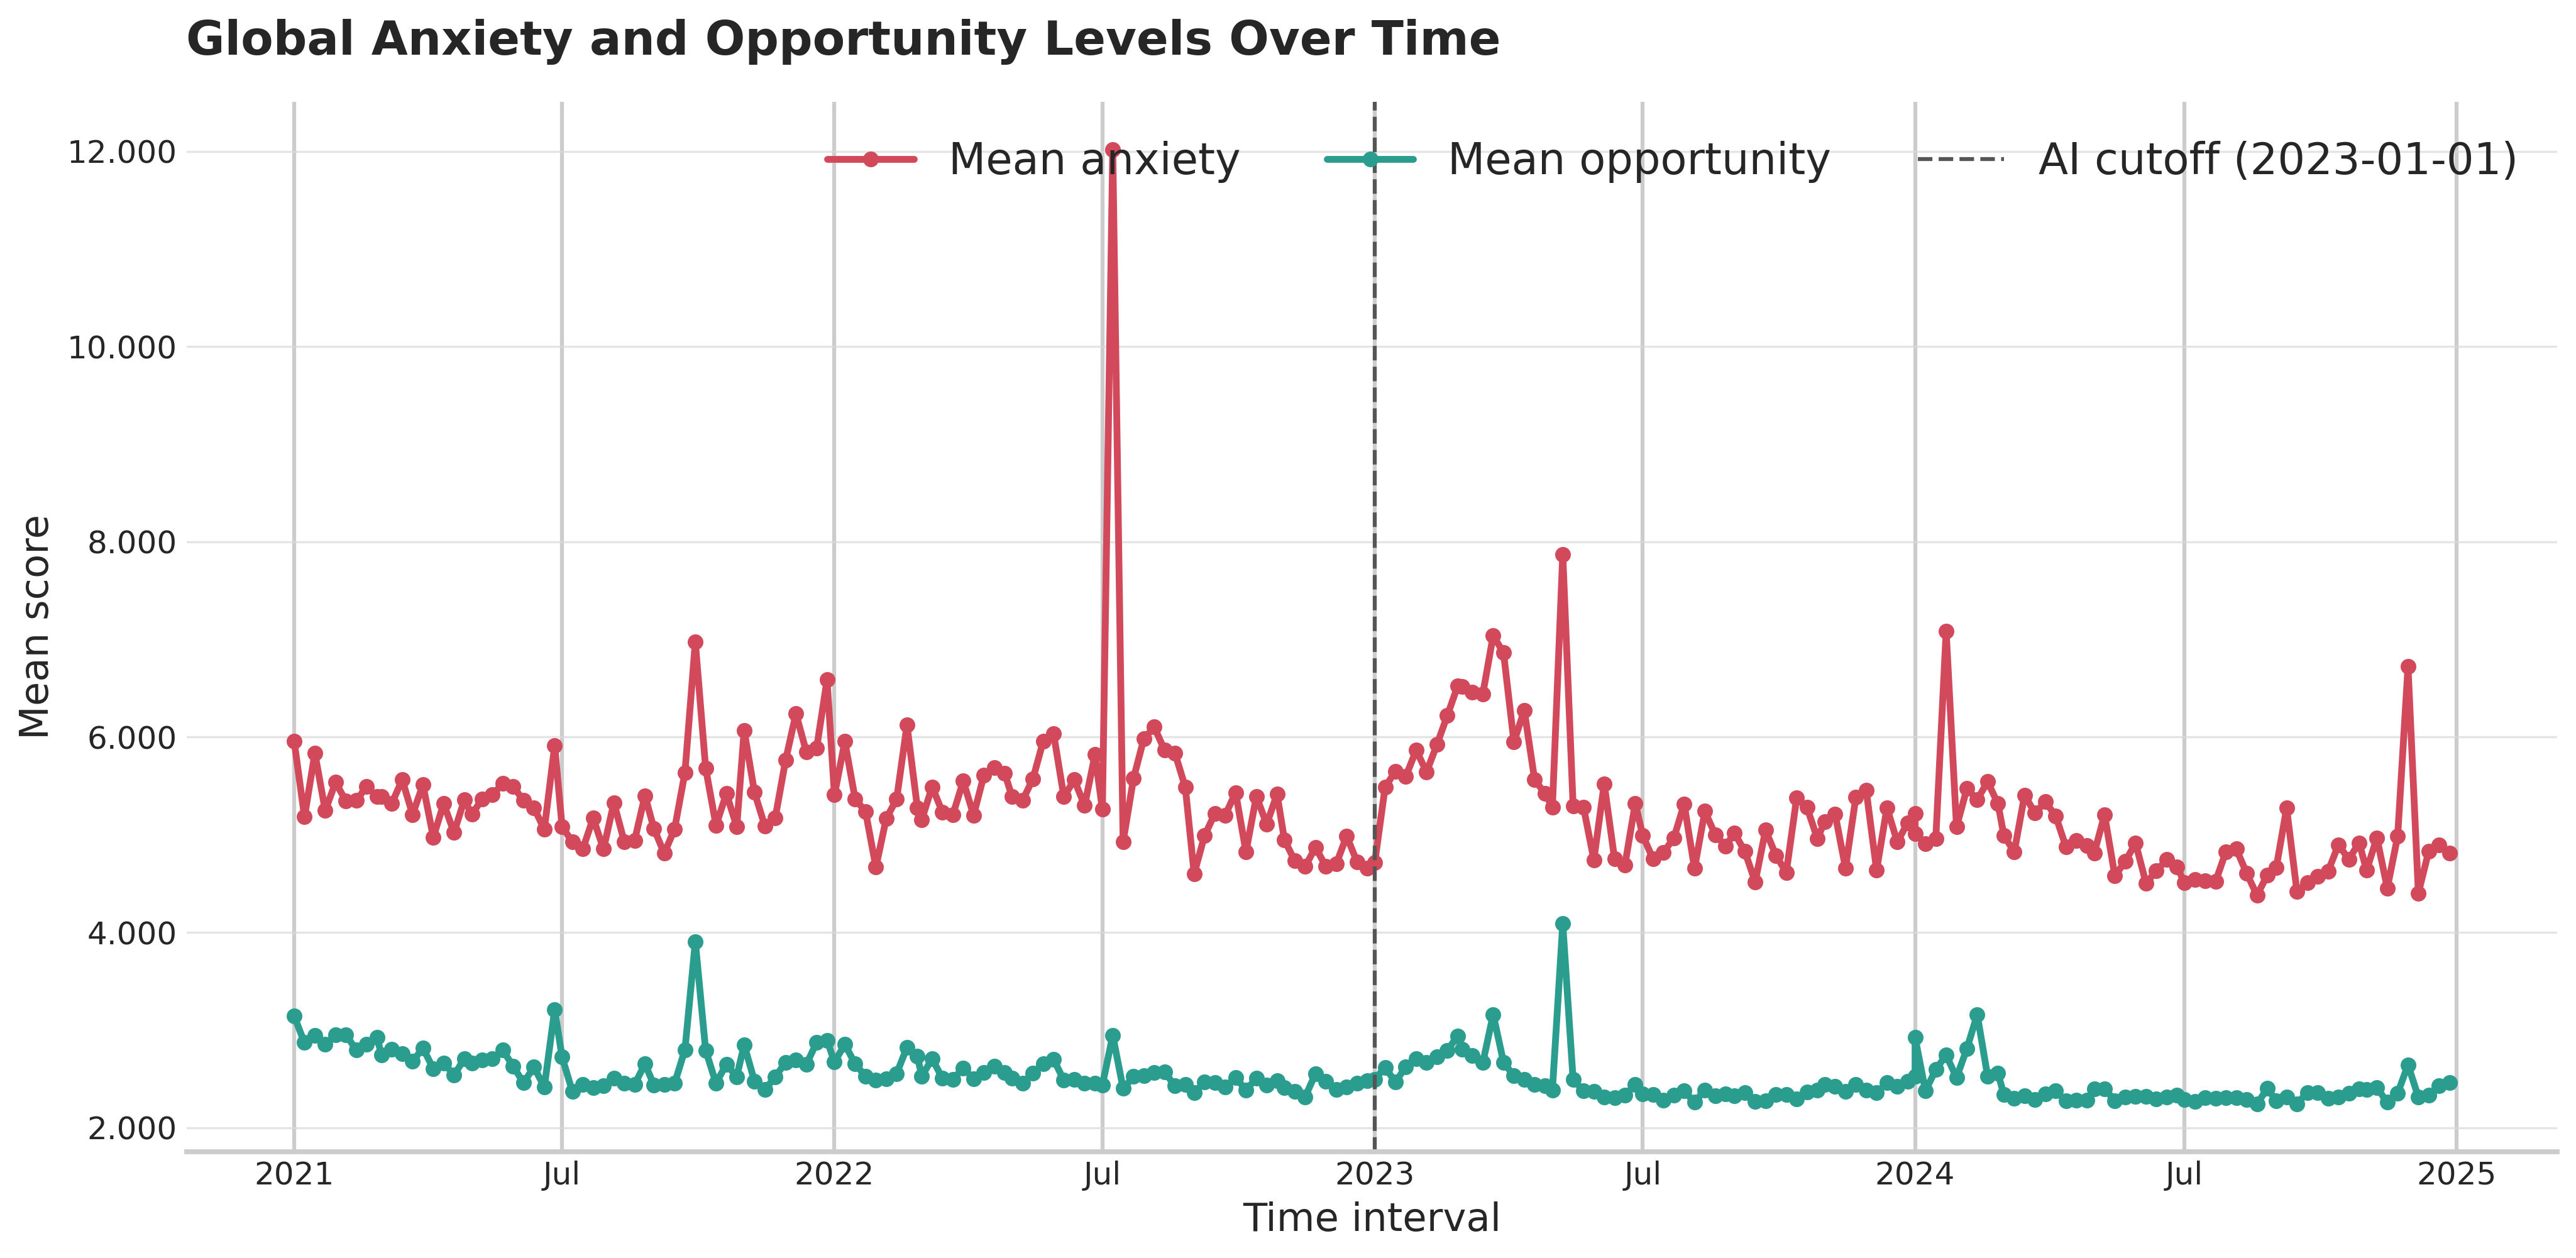
\includegraphics[width=0.8\textwidth]{global_temporal_anxiety_opportunity.png}
\caption{Weekly global anxiety and opportunity scores. The dashed line marks
the operational cutoff; the pre-cutoff peak cautions against a causal reading
of the two-period comparison.}
\label{fig:temporal}
\end{figure*}

Table~\ref{tab:global} shows that global labor-market framing became less
emotionally intense after the cutoff. Mean anxiety decreased from 6.341 to
5.902 (6.9\%), mean opportunity decreased from 2.785 to 2.592 (6.9\%), and
the anxiety-opportunity gap decreased from 4.617 to 4.225 (8.5\%).
At the same time, the summed article counts across all location--theme
groups increased by 99.9 million (13.9\%). Because one article may contribute
to multiple groups, this increase reflects greater indexed coverage rather
than 99.9 million additional unique articles.

Welch tests reject equal period means for anxiety ($t=-88.44$), opportunity
($t=-124.40$), and the gap ($t=-64.04$), all $p<.001$. 
Figure~\ref{fig:temporal} shows substantial variation within both periods and
no clear discontinuity at January 1, 2023. The largest anxiety peak occurred
before the cutoff, in July 2022 (12.017), whereas the largest after-period
peak occurred in May 2023 (7.871). 

\subsection{RQ2: Cross-Country Emotional Variation}

\begin{figure*}[!t]
\centering
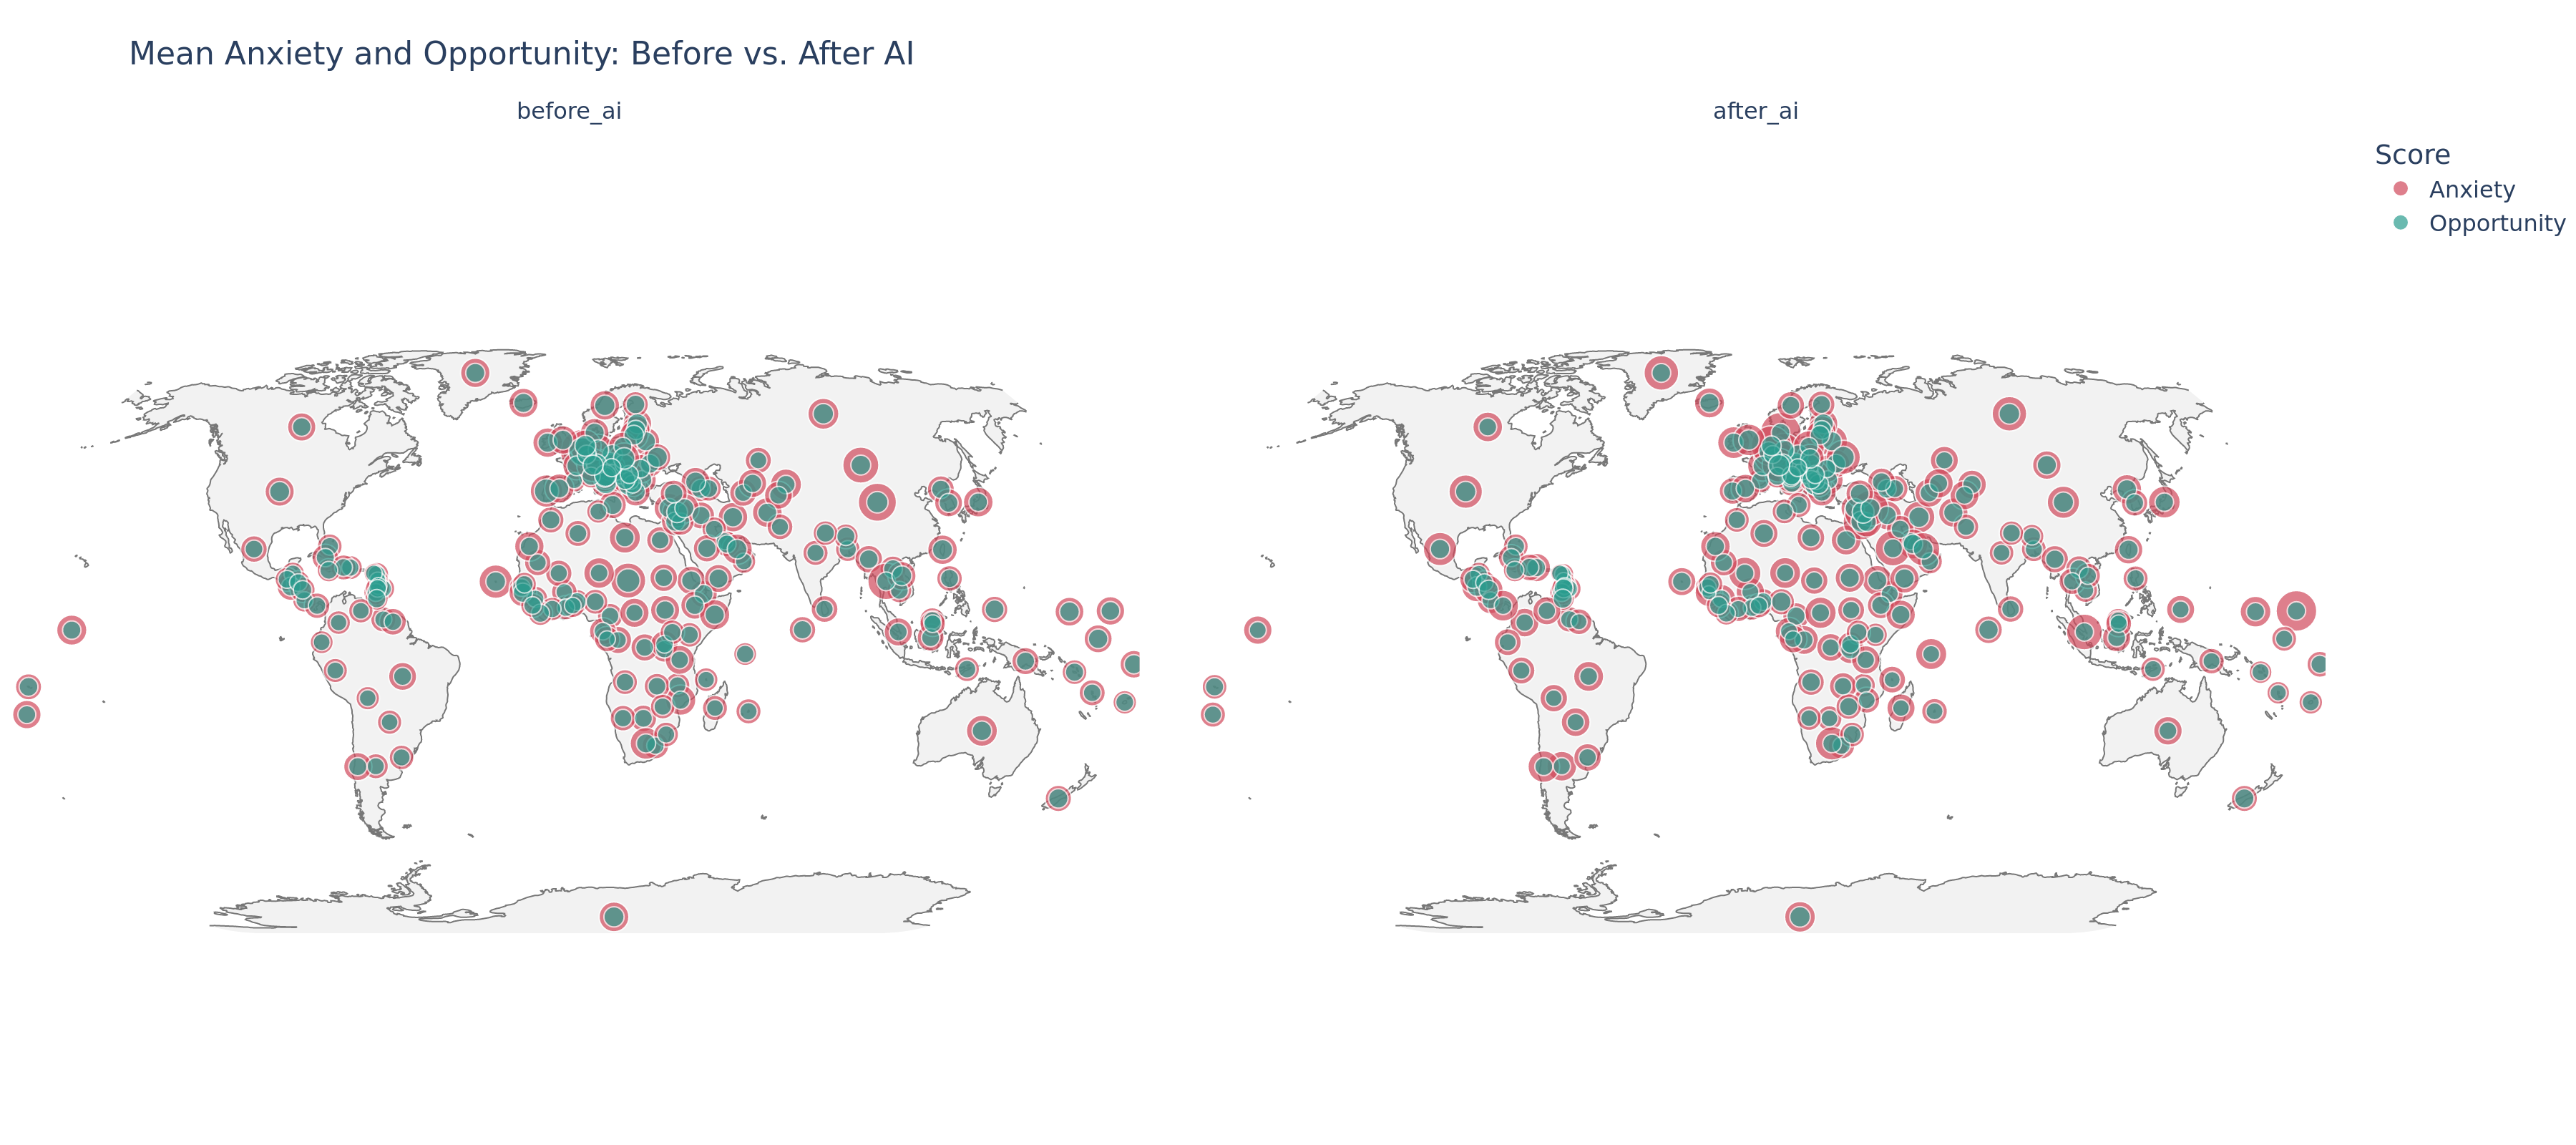
\includegraphics[width=0.96\textwidth]{country_temporal_changes_pydeck.png}
\caption{Country-level mean anxiety and opportunity scores before and after
the cutoff. Marker size represents the mean score; red denotes anxiety and
green denotes opportunity.}
\label{fig:country-comparison}
\end{figure*}

\begin{table}[t]
\caption{Direction of country-level score changes}
\label{tab:geography}
\centering
\scriptsize
\resizebox{\columnwidth}{!}{%
\begin{tabular}{rrrrrrr}
\toprule
\shortstack{Countries\\analyzed} &
\shortstack{Anxiety\\increased} &
\shortstack{Anxiety\\decreased} &
\shortstack{Opportunity\\increased} &
\shortstack{Opportunity\\decreased} &
\shortstack{Same\\direction} &
\shortstack{Opposite\\directions} \\
\midrule
197 & 122 & 75 & 78 & 119 & 137 & 60 \\
\bottomrule
\end{tabular}
}
\end{table}

The global decline was not geographically uniform. As shown in
Fig.~\ref{fig:country-comparison} and Table~\ref{tab:geography}, anxiety
increased in 122 of 197 countries and decreased in 75, whereas opportunity
increased in 78 countries and decreased in 119. 

Changes in anxiety and opportunity were positively correlated across
countries ($r=0.572$). Both scores increased in 70 countries and decreased in
67, giving 137 countries in which they moved in the same direction, compared
with 60 in which they moved in opposite directions. At the marginal level, anxiety
increased in most countries while opportunity decreased in most countries,
but the frequent co-movement of the two scores shows that anxious and
opportunity-oriented framing are not strict opposites.

\subsection{RQ3: Location Similarity and Polarization}

\begin{figure*}[!t]
\centering
\includegraphics[width=0.96\textwidth]{location_similarity_networks.png}
\caption{Location-similarity networks before and after the cutoff. Nodes
represent the 20 highest-volume locations in each period, and edge width
represents the emotional-overlap similarity score. The layout supports visual
comparison only; interpretation is based on the edge weights.}
\label{fig:similarity-networks}
\end{figure*}

\begin{figure*}[!t]
\centering
\includegraphics[width=0.8\textwidth]{location_similarity_score_differences.png}
\caption{Largest increases and decreases in pairwise emotional-similarity
scores among the 153 location pairs observed in both periods. Positive values
indicate convergence and negative values indicate divergence.}
\label{fig:similarity-differences}
\end{figure*}

The period networks each contain 20 locations and all 190 possible pairwise
edges; 18 locations occur in both periods, producing 153 directly comparable
pairs. Among these shared pairs, mean similarity declined from 49.326 to
48.581, a decrease of 1.5\%. The aggregate shift was therefore toward slightly
less similar emotional framing. It was not uniform: 80 pairs became more
similar and 73 became less similar. Figure~\ref{fig:similarity-networks}
provides the complete weighted-network view for each period, while
Fig.~\ref{fig:similarity-differences} isolates the largest matched-pair
changes.

Figure~\ref{fig:similarity-differences} shows that the largest convergence was
Russia--Ukraine (+97.7\%), followed by Israel--Russia (+74.9\%) and
Israel--Ukraine (+72.7\%). The largest divergence was China--Germany
(-30.9\%), followed by China--Vietnam (-26.8\%) and Germany--Vietnam
(-26.8\%).

\section{Conclusions}

\subsection{Discussion}

The findings indicate that the emotional framing of global labor-market 
news became less intense after the January 1, 2023 cutoff. 
Mean anxiety and opportunity scores each declined by approximately 6.9\%, 
while the anxiety-opportunity gap narrowed by 8.5\%. 
However, the weekly time series remained highly variable and 
showed no abrupt discontinuity at the cutoff. 
These global trends also concealed substantial geographic variation: 
anxiety increased in 122 of 197 countries, 
while opportunity increased in 78, and changes in the two measures 
were positively correlated. At the network level, average emotional 
similarity among comparable location pairs decreased by only 1.5\%. 
Since 80 pairs converged and 73 diverged, the results suggest a 
selective reconfiguration of emotional relationships across locations 
rather than widespread polarization.

A comparable survey covering a similarly broad set of countries 
throughout the entire study period is not available and would 
be difficult to construct retrospectively. 
Large-scale news data therefore provide a useful, 
time-stamped source for systematically comparing emotional framing across 
locations and periods using a consistent procedure.


\subsection{Limitations}

Several limitations should be acknowledged. 
First, the analysis treats the labor market as a broad domain and 
does not distinguish among industries, occupations, skill levels, 
or employment arrangements. 
As a result, the aggregate findings may obscure meaningful 
variation across labor-market segments. 
Second, the study does not provide detailed economic or political analyses 
of individual countries. 
Factors such as unemployment, inflation, regulation, elections, 
armed conflict, and differences in media systems may have contributed 
to the observed geographic and temporal patterns. 
Third, the analysis does not establish a causal relationship between the 
diffusion of generative AI and changes in emotional framing or 
cross-location similarity. 

\subsection{Future Work}

Future research should disaggregate labor-market discourse 
by industry, occupation, skill level, and employment arrangement 
to identify variation across labor-market segments. 
It could also incorporate economic, political, and survey data.
In addition, causal inference methods could be applied 
to better identify the factors driving the observed changes.


\section*{Acknowledgment}

The author acknowledges GDELT, the course staff, and Ben-Gurion University
computing resources. OpenAI ChatGPT and Codex assisted with brain storming, 
coding and linguistic editing. The author verified the results and
responsible for the analysis and conclusions.


\FloatBarrier
\clearpage
\twocolumn[]
\bibliographystyle{IEEEtran}
\bibliography{references}

\end{document}
